\section{Le 2.3}
The system is defined as 
\begin{align*}
    \dot x &= 1 & y = h(x)
\end{align*}

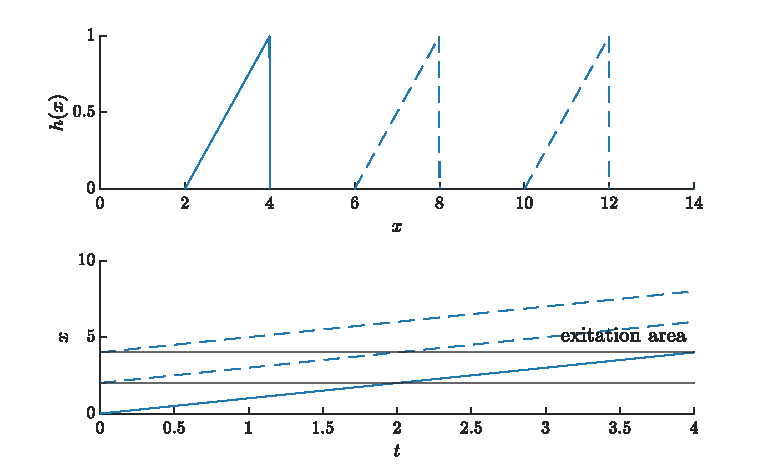
\includegraphics{figures/ex2_3.pdf}

(a) $\mathcal{M} \subset \left(0, 4\right)$ \hspace{4em} \textbf{Weakly observable}. 

\fbox{\parbox{0.98\textwidth}{
    At $x < 2$, $h(x) = 0$ and thus not locally observable. However, $\forall t>=2,\, h(x) = k\,x$ and becomes observable.
}}
% \begin{tabular}{c|c|c}
%      & $\mathcal{M} = \left(0, 4\right)$ & \\
%     \hline
%     locally observable & \textbf{No} & not obs. at $x < 2$, $h(x) = 0$\\ 
%     weakly observable & \textbf{Yes} & obs. at $x \approx 2$, $h(x) = 0$ \\
%     locally weakly observable & \textbf{No} 
% \end{tabular}

(b) $\mathcal{M} = \left(2, 4\right)$ \hspace{4em} \textbf{Locally observable}. 

\fbox{\parbox{0.98\textwidth}{
    $x$ is uniquly isolable for all $\mathcal{U} \subset \mathcal{M}$.
}}

% \begin{tabular}{c|c|c}
%     & $\mathcal{M} = \left(2, 4\right)$ & \\
%    \hline
%    locally observable & \textbf{Yes} & \\ 
%    weakly observable & \textbf{Yes} & \\
%    locally weakly observable & \textbf{Yes} 
% \end{tabular}

(c) $\mathcal{M} = \mathcal{R}^+\ '\cdots'$ \hspace{4em} \textbf{Weakly observable}. 
% \begin{tabular}{c|c|c}
%     & $\mathcal{M} = \mathcal{R}^+\ '\cdots'$ & \\
%    \hline
%    locally observable & \textbf{No} & not obs. at $x < 2\cdots$, $h(x) = 0$\\ 
%    weakly observable & \textbf{Yes} & no unique solutions even for $x < 2$, indistinguishable\\
%    locally weakly observable & \textbf{No} 
% \end{tabular}
% It is still observable in some space [0,2]

\fbox{\parbox{0.98\textwidth}{
    $ 2 \geq t \leq 4,\, h(x) = k\,x$ and becomes observable.
}}

Note:

\fbox{\parbox{0.98\textwidth}{
    if $h(x)$ is a sawtooth waveform, then the system is \textbf{locally weakly observable}.
}}